\documentclass[12pt,a4paper]{article}
\usepackage[utf8]{inputenc}
\usepackage[spanish]{babel}
\usepackage{amsmath}
\usepackage{amsfonts}
\usepackage{amssymb}
\usepackage[left=2cm,right=2cm,top=2cm,bottom=2cm]{geometry}
\usepackage[T1]{fontenc}
\usepackage{titlesec}
\usepackage{hyperref}
\hypersetup{
    colorlinks=true,
    linkcolor=blue,
    urlcolor=red,
    pdftitle={Tarea 4 Viajero búsqueda local},
    }
\author{Lic. Arnoldo Del Toro Peña}
\title{Tarea 4: Algoritmo Set Covering \\ Búsqueda local}
\date{\today}
\usepackage{natbib}
\bibliographystyle{dinat}
\usepackage{graphicx}
\titleformat{\section}[display]
{\normalfont}{\filcenter\small
\ SECCIÓN \thesection   }
{0.5pt}{\Large\bfseries\filcenter  \hrulefill \\ }

%% %--
%\usepackage{titlesec}
%\titleformat{\section}[frame]{\normalfont} %
%{\filright\footnotesize\enspace SECCIÓN \thesection\enspace} %
%{8pt}{\Large\bfseries\filcenter} %
%%-




\begin{document}

\maketitle



\thispagestyle{empty}
\begin{abstract}
    Uso de un método metahurístico con una implementación de búsqueda local para la solución a un problema del viajero utilizando programación en python.
\end{abstract}
{\centering \textit{Palabras clave: python,viajero, metahurística, búsqueda,local.}}
\section{Introducción}
En este documento se presentarán los resultados a las instancias obtenidas, se compararán con los resultados óptimos que se presentan a continuación:
\begin{table}[h!]
\centering
\begin{tabular}{|c|c|c|c|c|}
\hline
\multicolumn{1}{|l|}{\textbf{Instancias de Prueba}} & \multicolumn{1}{l|}{\textit{Nombre de la instancia}}  & \multicolumn{1}{c|}{\textit{nodos}} & \textit{Óptimo} \\ \hline
\textit{76}                                          &  pr76.tsp                                & 76                            & 108159            \\ \hline
\textit{105}                                          & lin105.tsp                                 & 105                            & 14379             \\ \hline
\textit{280}                                          & a280.tsp                                 & 280                           &2579            \\ \hline
\textit{130}                                          & ch130.tsp                                 & 130                            & 6110             \\ \hline
\textit{225}                                          & tsp225.tsp                                 & 225                            & 3919             \\ \hline

\end{tabular}
\end{table}

Más adelante analizaremos las diferencias entre estos resultados y los que obtuvimos.

\section{Descripción}
 El algoritmo que se pidió fue el del nodo más cercano el cual se menciona en el siguiente diagrama:
 \begin{figure}[ht]
    \centering
    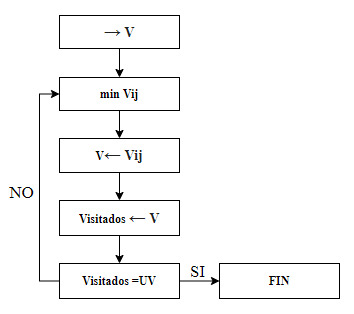
\includegraphics[scale = 0.5]{diagrama.jpeg}
    \caption{Diagrama}     
 \end{figure}
 \newpage Una breve explicación del digrama anterior; podemos observar que una vez que marcamos el nodo se exploran sus conexiones con nodos no marcados y se selecciona el menor y esto se repite hasta marcar todos los nodos.
 \newline Posteriormente a esto se implementó una búsqueda local, en el cual se intercambiaron dos nodos, se almacenó en una variable delta y se comparó con el valor antes del intercambio, si este mejoraba la solución se mantenía el cambio, de otro modo no se hacía el cambio, en el código
 se imprime un mensaje si se realiza este mismo, al final el código imprime el mejor valor objetivo obtenido y su respectiva ruta junto con el valor antes de la búsqueda local.  
\section{Descripción del algoritmo}
 El algoritmo se finaliza cuando todos los nodos estan marcados y tenemos que agregar el nodo inicial al final para poder cerrar el recorrido.Podemos enumerar sus pasos de la siguiente manera:
\begin{enumerate}
    \item Elección de un vértice arbitrario respecto al vértice actual.
    \item Descubra la arista de menor distancia que ya este conectada al vértice actual y a un vértice no visitado V.
    \item Convierta el vértice actual en V.
    \item Marque V como visitado.
    \item Si todos los vértices del dominio estuvieran visitados, cierre el algoritmo.
    \item Vaya al paso 2
\end{enumerate}
El algoritmo de búsqueda local sigue los siguientes pasos:
\begin{enumerate}
    \item Seleccionamos los nodos a intercambiar.
    \item Si los nodos son adyacentes entonces: calculamos el delta de la siguiente manera $$C_{act} = C_{i-1,i}+C_{i,j}+C_{j,j+1}$$, $$C_{nue} = C_{i-1,j}+C_{j,i}+C_{i,j+1}$$ $$\delta = C_{act} - C_{nue}$$
    \item Si no, calculamos el delta de la siguiente manera: $$C_{act} = C_{i-1,i}+C_{i,i+1}+C_{j-1,j}+C_{j,j+1}$$, $$C_{nue} = C_{i-1,j}+C_{j,i+1}+C_{j-1,i}+C_{i,j+1}$$ $$\delta = C_{act} - C_{nue}$$
    \item Si $\delta \geq 0$ entonces intercambiamos los nodos.
    \item Si no hemos hecho esto para todos los nodos regresamos al paso 1. 
\end{enumerate}
\section{Implementación} 
El algoritmo se programó en lenguaje python con referencias en \cite{van1991guia}, \cite{van2017tutorial} y \cite{chun2001core}, y se puede verificar en el siguiente repositorio de: \href{https://github.com/arnoldae9/PycharmProjects.git}{git-hub}.

\section{Resultados} 
Los resultados se pueden ver en el mismo enlace de git-hub, en los documentos txt, sin embargo se presentarán a continuación en una forma más ordenada:
\\ Los viajes los podemos encontrar en los archivos 76.txt, 105.txt, 280.txt, 130.txt, 225.txt disponibles en el repositorio de Git mencionado en la parte de arriba. 
\begin{table}[h!]
    \centering
    \resizebox*{15 cm}{!}{\begin{tabular}{|c|c|c|c|c|c|c|c|}
        \hline
        \multicolumn{1}{|l|}{\textbf{Instancias de Prueba}} & \multicolumn{1}{l|}{\textit{Nombre de la instancia}}  & \multicolumn{1}{c|}{\textit{nodos}} & \textit{Óptimo} & \textit{Aproximado} &\textit{Búsqueda local}      & \textit{error búsqueda \%}       \\ \hline
        \textit{76}                                          &  pr76.tsp                                & 76                            & 108159                            &153461.92            &132518.35      & 22.52 \%       \\ \hline
        \textit{105}                                          & lin105.tsp                                 & 105                            & 14379                         &20362.75            &20055.21      & 39.47 \%      \\ \hline
        \textit{130}                                          & ch130.tsp                                 & 130                            & 6110                           &7575.28            &7478.11      & 22.39 \%     \\ \hline
        \textit{225}                                          & tsp225.tsp                                 & 225                            & 3919                          &4774.84            &4598.00      & 17.32 \%     \\ \hline
        \textit{280}                                          & a280.tsp                                 & 280                           & 2579                                &3338.27            &3238.81      &  25.58 \%            \\ \hline
        &&&&& \bfseries{Promedio:} & 25.45 \%  \\ \hline
        \end{tabular}}
    \end{table}
\section{Mejoras}
La idea de seleccionar el nodo mas cercano al nodo actual depende totalmente del nodo inicial; una idea que tuve fue ir tomando como nodo inicial cada uno de los nodos del viaje, entonces al final tendremos varias soluciones de las cuales podemos tomar la mejor opción.
\newline Se mejoró la solución con un algoritmo de búsqueda local, utilizando el mismo nodo y la solución obtenida del algoritmo anterior.
\section{Conclusiones} 
Si observamos los porcentajes, los porcentajes mejoraron en un porcentaje, ninguna opción, aun así, personalmente los \,  \% de errores son demasiados altos, sin duda tenemos que buscar mejorar el algoritmo o buscar una mejora al algoritmo de búsqueda local.
\newpage
\bibliography{biblio}
\end{document}
